\documentclass[]{report}

\usepackage{graphicx}
\usepackage{Bookmark}
\usepackage{listings}

%opening
\title{Testing Document}
\author{Grant Louat}

\begin{document}

\maketitle

\newpage

\begin{abstract}
This document details the testing of all functions, and their current state. Each function will be tested in isolation. This document should detail by what criteria the function has been deemed correct, the date and who did the testing. It should also have a listing of the working code so there is no confusion over different versions. This will quickly tell everyone which functions have been confirmed correct, and the rigour to which that assertion was made. It will also tell them when it was confirmed in case they have been working on a local copy of the code, and who deemed it correct in case they have questions. This document should also have a description of the function so that people know what the function should be doing when it is working.\newline
The document deals only with the isolation testing of each function. The functions will also need to be tested in an integration phase later. \newline
WARNING: DO NOT INCLUDE ANYTHING IN THIS DOCUMENT UNLESS YOU ARE CERTAIN THAT IT IS COMPLETELY ERROR FREE! \newline Even if it is a simple one line function there could be a type issue or something. Anything document will be assumed working, and if a single error remains it will nullify the entire document. If a function is too large or complex to test and verify in complete certainty then it should be split into smaller functions to solve parts of the problem. Make sure also to include WHY you verified the function correct, as your rigour may not meet the standard of someone else's.
\end{abstract}

\newpage
\section{Common}

\subsection{DIV\_X Macros:}
\subsubsection{Status:}
Working as of 11:30 25/9/2014 - Grant

\subsubsection{Description:}
This set of Macros are designed to divide an integer by a power of two.

\subsubsection{Criteria:}
The value of 1024 was tested for each of the macros, and due to the simplicity and nature of the macros no other values need be tested.

\subsubsection{Working code:}
\begin{lstlisting}
#define DIV_2(v) ((v) >> 1)       //Divide by 2
\end{lstlisting}

\subsection{SWAP Macro}
\subsubsection{Status:}
Working as of 10:00pm 6/10/2014 - Grant

\subsubsection{Description:}
This macro provides an efficient way of swapping the values in two variables using xor operations.

\subsubsection{Criteria:}
The macro was tested on the values x = 7, y = 3, the macro returned x = 3, y = 7. As this was the expected result and any error in the macro would have manifested an error in the result, the macro was thus assumed to be correct.

\subsubsection{Working Code:}
\begin{lstlisting}
#define SWAP(x, y) (y = (y ^ (x = (x ^ (y = (x ^ y))))))
\end{lstlisting}

\newpage
\section{Temperature Module:}

\subsection{ReadTempx2:}

\subsubsection{Status:}
Currently untested as of 8am 26/9/14 - Grant

\subsubsection{Description:}
Returns the temperature (x2) in degrees Celsius by performing an A/D conversion on the analogue output from the temperature sensor.

\subsection{ReadTemp:}
\subsubsection{Status:}
Working as of 8am 26/9/2014 - Grant

\subsubsection{Criteria:}
This function was tested in isolation of the ReadTempx2, and the assertion only applies to this function. A ReadTempx2 stub function was written to simply return the value of 40 to test the ReadTemp function.

\subsubsection{Description:}
The function simply calls the ReadTempx2 function and divides the result by 2.

\subsubsection{Working Code:}
\begin{lstlisting}
unsigned char readTemp(void)
{
unsigned char temp;

//Read the temperature from the x2 function
temp = readTempx2();

//Divide the temp by two and return the result
return DIV_2(temp);
}
\end{lstlisting}

\subsection{RawTemp:}

\subsubsection{Status:}
Working as of 8:30am 26/9/2014 - Grant

\subsubsection{Criteria:}
The function was tested in isolation of the ReadTemp functions. A dummy function placed the value of 60 into the lastTempx2 variable, and the RawTemp function worked as described.

\subsubsection{Description:}
This function returns the uncalibrated result of the last temperature read. E.g. the raw sensor output. A temperature read is performed by either a ReadTemp or ReadTempx2 call. \newline:
This function cannot be completely tested in isolation as it requires an external static declaration of the lastTempx2 variable. It also requires the ReadTemp and ReadTempx2 functions to write to this variable when they perform a read.

\subsubsection{Working Code:}
\begin{lstlisting}
unsigned char rawTemp(void)
{
return DIV_2(lastTempx2);
}
\end{lstlisting}

\subsection{Calibrate Temp:}
\subsubsection{Status:}
Working as of 10:30am 26/9/2014 - Grant

\subsubsection{Description:}
Calibrates the last temperature read to the passed reference value by updating a static variable.

\subsubsection{Criteria:}
This function was tested in isolation of the readTemp functions. a dummy readTempx2 function which just returned 15deg (and set the static variable) was written, and the calibration function called to calibrate it to 20 deg, and then 10 deg. In both cases a second call of readTempx2 returned the desired value even though the 'raw data' was simply hard coded in.

\subsubsection{Working Code:}
\begin{lstlisting}
void calibrateTemp(unsigned char reference)
{
calibration_offset = 2 * (reference - DIV_2(lastTempx2));
}
\end{lstlisting}

\subsection{GetTemp:}

\subsubsection{Status:}
Working as of 10:30 26/9/2014 - Grant

\subsubsection{Description:}
Returns the result of the last temperature read.

\subsubsection{Criteria:}
This is just an accessor function, so it simply returns the value of a static variable.

\subsubsection{Working Code:}
\begin{lstlisting}
unsigned char getTemp(void)
{
return DIV_2(lastTempx2);
}
\end{lstlisting}

\newpage
\section{Range}

\subsection{SPD\_SND Macro}
\subsubsection{Status:}
Working as of 10:30 25/9/14 - Grant

\subsubsection{Description:}
This macro performs a linear approximation of the given function for the sake of computational efficiency. This means the computations performed are very different from the function provided, but the results closely approximate those of the actual function within the relevant range. See Fig. \ref{fig:SND_comp} for a comparison.

\subsubsection{Criteria:}
Each temperature from 0 to 100 deg C was tested and compared to the actual formula result. There is some deviation, but not much to make a significant difference. See Fig. \ref{fig:SND_comp}.\newline 

\subsubsection{Working Code:}
\begin{lstlisting}
#define SPD_SND(T) (DIV_1024(T * (unsigned int)614) + 331)
\end{lstlisting}

\begin{figure}
	\centering
	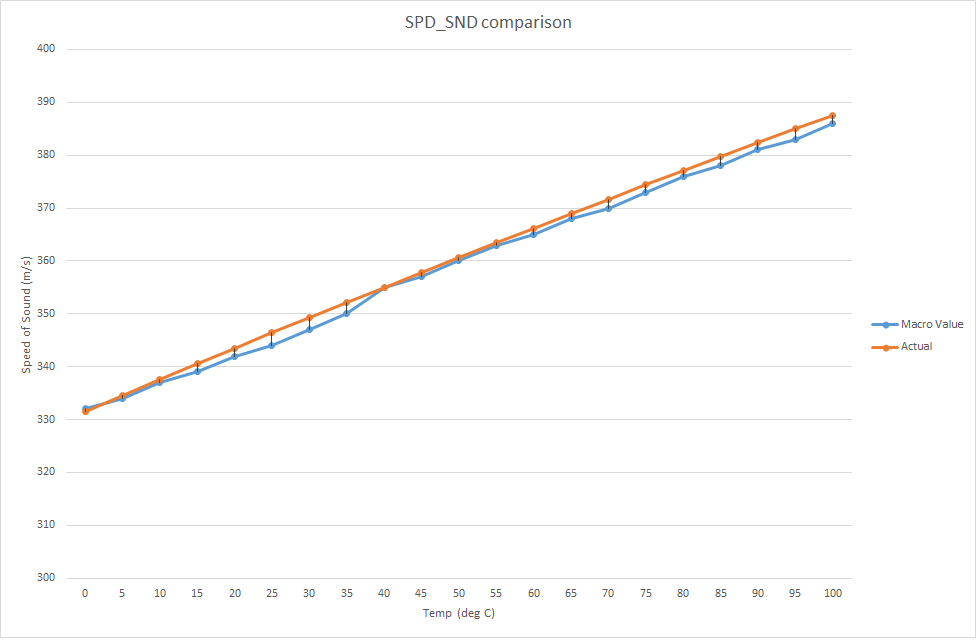
\includegraphics[width=0.7\linewidth]{SND_comp}
	\caption{Comparison between SPD\_SND() Macro output and actual function value}
	\label{fig:SND_comp}
\end{figure}

\subsection{IR\_CONV Macro:}
\subsubsection{Status:}
Working as of 1:40pm 30/9/2014 - Grant \newline
As of 13/10/2014 The calibration on the minimal board seems to differ. As of yet we have no idea why, and mean to re-calibrate it

\subsubsection{Description:}
This macro converts the AD result into a range in mm, based on experimental readings from the IR Sensor.

\subsubsection{Criteria:}
This macro has been tested with a range of different input values. Each input returned a distance within a couple of centimetres of the experimental data (which was within the experimental error). See Fig. \ref{fig:IRExperimentalData} for the sensor profile.

\begin{figure}
\centering
\includegraphics[width=1\linewidth]{"IR Experimental Data"}
\caption{IR Experimental Data - Sensor output profile}
\label{fig:IRExperimentalData}
\end{figure}


\subsubsection{Working Code:}
\begin{lstlisting}
#define IR_CONV(ad) ((unsigned long)237411 / (ad) - 65)
\end{lstlisting}

\subsection{US\_CONV}
\subsubsection{Status:}
Currently working as of 3:15 13/10/2014 - Grant

\subsubsection{Description:}
This function converts a timing value returned by the input capture into an actual range for the ultrasonic sensor. \newline
NOTE: This macro was designed for, and tested on the MINIMAL board. The ticks on the demo board will be 4x longer (as the clock is 4MHz instead of 10MHz). If using the demo board, multiply the system ticks by 4.

\subsubsection{Criteria:}
This function has been tested at different ranges, by comparing the range result to the measured distance to a target. The function was created from experimental data and a linear fit as seen in Fig. \ref{fig:UltrasonicProfile}.

\begin{figure}
\centering
\includegraphics[width=0.7\linewidth]{"Ultrasonic Profile"}
\caption{Ultrasonic Range profile. The measured distance against the time delay (in system ticks at 2.5MHz)}
\label{fig:UltrasonicProfile}
\end{figure}


\subsection{calibrateRange:}
\subsubsection{Status:}
Currently Untested as of 12:10pm 10/10/2014 - Grant

\subsubsection{Description:}
Calculates the offset to calibrate a calculated range to an argument.

\subsubsection{Criteria:}

\subsection{rawRange:}
\subsubsection{Status:}
untested as of 11am 26/9/2014 - Grant

\subsubsection{Description:}
Accessor function - simply returns the uncalibrated sensor output from the last range calculation.

\subsubsection{Criteria:}

\subsection{range:}
\subsubsection{Status:}
Untested as of 11am 26/9/14 - Grant

\subsubsection{Description:}
This function performs a read of both the ultrasonic and IR sensors, fuses them and calibrates the result. The current version simply averages the IR and ultrasonic ranges as an initial fusion method.

\subsubsection{Criteria:}

\subsection{rangeIR:}
\subsubsection{Status:}
Untested as of 11am 26/9/14 - Grant

\subsubsection{Description:}
This function performs a read of the IR sensor, calibrates it and returns the result.

\subsubsection{Criteria:}
This function has been tested with a range of different ranges (using a book and measuring the distance from the IR sensor with a tape measure). In each case the calculated distance was within around 30mm of the actual distance.

\subsubsection{Working Code:}
\begin{lstlisting}
unsigned int rangeIR(void)
{
unsigned int ad_result;
unsigned int range;

ad_result = sampleIR(10);

//Return 0 if there is no target detected
if (ad_result < 100) return 0;

//Convert voltage (0-5v) into range (mm)
range = IR_CONV(ad_result);

return range + calibration_offset_IR;
}
\end{lstlisting}

\subsection{SampleIR:}
\subsubsection{Status:}
Working as of 4pm 30/9/2014 - Grant

\subsubsection{Description:}
This function performs a specified number of reads of the IR sensor and returns the average.

\subsubsection{Criteria:}
This function has been tested using different ranges for the IR sensor, and each time it has returned the (approximately) correct result.

\subsubsection{Working Code:}
\begin{lstlisting}
unsigned int sampleIR(char numSamples)
{
unsigned long int sum = 0;
unsigned int temp;
char i = 0;

//Multiplex onto the IR sensor
SetChanADC(ADC_IR_READ);

//Perform numSamples samples
for (i = 0; i < numSamples; i++)
{
ADCON0bits.GO = 1;
while (ADCON0bits.GO_NOT_DONE);
temp = ADRES >> 6;
sum += temp;
}

//Average all samples taken
temp = sum / (unsigned int)numSamples;
return temp;
}
\end{lstlisting}

\subsection{rangeUS:}
\subsubsection{Status:}
Working as of 13/10/2014 - Grant

\subsubsection{Description:}
This function performs a read of the Ultrasonic sensor (if not already started), calibrates it and returns the result.

\subsubsection{Criteria:}
This function has been tested over a number of different ranges, and a calibration curve fitted as seen in Fig. \ref{fig:UltrasonicProfile}.


\subsection{ConfigureAD:}
\subsubsection{Status:}
Working as of 4pm 30/9/2014 - Grant

\subsubsection{Description:}
This function configures the ADC so that it can subsequently be used (immediately after).

\subsubsection{Criteria:}
There are few testing methods that can be applied to this function in isolation, but after running this function the ADC sampling functions are running properly, so we assume that it is correct. Any future ADC problems should begin with an analysis of this function.

\subsubsection{Working Code:}
\begin{lstlisting}
void configureAD(void)
{
int i = 0;
TRISA = 0xFF;

//Write the configuration values into the configuration registers
ADCON1 = 0x8E;
ADCON0 = 0x41;

//Arbitrary wait period to allow the ADC to initialise
for (i = 0; i < 1000; i++);
}
\end{lstlisting}

\subsection{BeginUS:}
\subsubsection{Status:}
Untested as of 12pm 26/9/2014

\subsubsection{Description:}
This function begins an ultrasonic scan and returns. The returning echo will be serviced by an interrupt and the value will be stored in the range module for the next rangeUS call.

\subsection{rangeISR:}
\subsubsection{Status:}
Untested as of 12pm 26/9/2014 - Grant

\subsubsection{Description:}
This function acts as the service routine for the range module. The exact function will depend on the implementation of the range module and what interrupts are used.

\subsubsection{Criteria:}

\newpage
\section{Tracking}

\subsection{ConfigureBase:}
\subsubsection{Status:}
Currently incomplete and untested as of 12:15pm 26/9/2014 - Grant

\subsubsection{Description:}
This function configures the pan tilt mechanism (which is acting as the base) so that it is ready for initial use.

\subsubsection{Criteria:}

\subsection{Search:}
\subsubsection{Status:}
Currently incomplete and untested as of 12:15pm 26/9/2014 - Grant

\subsubsection{Description:}
This function increments the pan tilt mechanism in a search pattern.

\subsubsection{Criteria:}

\subsection{trackingISR:}
\subsubsection{Status:}
Untested as of 1:20pm 26/9/2014 - Grant

\subsubsection{Description:}
This function acts as the ISR for the tracking module. The exact functionality will depend on what interrupts are associated with the tracking module, and how they are implemented.

\subsubsection{Criteria:}


\subsection{Edge:}
\subsubsection{Status:}
Currently untested as of 1:20pm 26/9/2014

\subsubsection{Description:}
This function finds the edge of the target in both the azimuth and declination degrees of freedom, and uses that to find (and track) the centre of the target. It could also be used as a rudimentary target verification based on the approximate size of the target.

\subsubsection{Criteria:}

\newpage
\section{Circular Buffers}
\subsection{Push Macro:}
\subsubsection{Status:}
Working as of 1:45pm 26/9/2014 - Grant

\subsubsection{Description:}
This macro pushes a byte onto a circular buffer. If the buffer is full then it begins overwriting the first data in the buffer.

\subsubsection{Criteria:}
This macro has been tested by pushing a byte onto an empty buffer, a partially filled buffer and a completely filled buffer. In each case the result was as documented.

\subsubsection{Working code:}
\begin{lstlisting}
#define push(byte, buf) buf.data[buf.head] = byte; if(full(buf)) incMod(buf.tail); incMod(buf.head)
\end{lstlisting}

\subsection{Pop Macro:}
\subsubsection{Criteria:}
Working as of 2:00pm 26/9/2014 - Grant

\subsubsection{Description:}
This macro pops a byte from a circular buffer. If the buffer is empty it returns whatever is in the first element location and does not change the pointers.

\subsubsection{Criteria:}
This macro has been tested with both empty and non-empty buffers and in each case it functions as documented.

\subsubsection{Working Code:}
\begin{lstlisting}
#define pop(buf) buf.data[buf.tail]; if (!empty(buf)) incMod(buf.tail)
\end{lstlisting}

\subsection{Init Macro:}
\subsubsection{Status:}
Working as of 2pm 26/9/2014 - Grant

\subsubsection{Description:}
This macro initialises a buffer before it can be used - It initializes the pointers to zero. This function will also completely clear a circular buffer.

\subsubsection{Criteria:}
This macro was tested by simply operating on a circularBuffer which was not previously initialized and making sure that it was subsequently initialised.

\subsubsection{Working Code:}
\begin{lstlisting}
#define init(buf) buf.head = 0; buf.tail = 0
\end{lstlisting}

\subsection{Peek Macro:}
\subsubsection{Status:}
Working as of 2:05pm 26/9/2014 - Grant

\subsubsection{Description:}
This macro returns the next byte that will be popped off the buffer, without removing that element from the buffer. If the buffer is empty it will simply return whatever happens to be in the first element.

\subsubsection{Criteria:}
This macro was tested by simply operating on a macro several times (between which push and pop operations were implemented) and making sure the correct thing was returned.

\subsubsection{Working Code:}
\begin{lstlisting}
#define peek(buf) buf.data[buf.tail]
\end{lstlisting}

\subsection{Full Macro:}
\subsubsection{Status:}
Working as of 2:05pm 26/9/2014 - Grant

\subsubsection{Description:}
This macro returns non-zero is the buffer is full, and zero otherwise.

\subsubsection{Criteria:}
This macro was tested by operating on a number of circular buffers, both full and not full (including empty), and in each case it returned the correct thing.

\subsubsection{Working Code:}
\begin{lstlisting}
#define full(buf) (buf.tail == (buf.head + 1) % BUFFERLENGTH)
\end{lstlisting}

\subsection{Empty:}
\subsubsection{Status:}
Working as of 2:10pm 26/9/2014 - Grant

\subsubsection{Description:}
This macro returns non-zero if the buffer is empty. Otherwise it returns zero.

\subsubsection{Criteria:}
This macro was tested on both empty and non-empty buffers, including full buffers. In all cases the macro returned the expected result.

\subsubsection{Working Code:}
\begin{lstlisting}
#define empty(buf) (buf.head == buf.tail)
\end{lstlisting}

\subsection{IncMod Macro:}
\subsubsection{Status:}
Working as of 2:30pm 26/9/2014 - Grant

\subsubsection{Description:}
This macro increments a buffer pointer and takes the modulus with the buffer length (defined by BUFFERLENGTH), which will loop back to zero, making the buffer circular.

\subsubsection{Criteria:}
This macro has been tested with a range of values from 0 to BUFFERLENGTH. In each case the macro returned the response as documented.

\subsubsection{Working Code:}
\begin{lstlisting}
#define incMod(ptr) (ptr = ++ptr % BUFFERLENGTH)
\end{lstlisting}

\newpage
\section{Serial}


\subsection{ConfigureSerial:}
\subsubsection{Remark:}
The baud rate set in this function is dependant on the clock speed of the processor. On the PICDEM board, and other PIC's this is 4MHz. On the minimal board it is a 10MHz clock.

\subsubsection{Status:}
Working as of 11:25am 1/10/2014 - Grant

\subsubsection{Description:}
This function sets up and configures the serial UART for communication to the remote terminal.

\subsubsection{Criteria:}
While there is no way to properly test this function in isolation the serial is working after this function has configured the serial.

\subsubsection{Working Code:}
\begin{lstlisting}
void configureSerial(void)
{
INTCONbits.GIEH = 1;
INTCONbits.GIEL = 1;
RCONbits.IPEN = 1;

//Initialise the serial buffers
init(transmit_buffer);
init(receive_buffer);
carriageReturn = 0;

//Open the USART module
OpenUSART(USART_TX_INT_ON & USART_RX_INT_ON & USART_BRGH_HIGH & USART_EIGHT_BIT & USART_ASYNCH_MODE, 25);
//OpenUSART(USART_TX_INT_ON & USART_RX_INT_ON & USART_BRGH_HIGH & USART_EIGHT_BIT & USART_ASYNCH_MODE, 64);
}
\end{lstlisting}

\subsection{Transmit:}
\subsubsection{Status:}
Working as of 11:20am 1/10/2014 - Grant

\subsubsection{Description:}
This function pushes a string onto the serial transmit buffer and enables the transmit interrupt to begin transmitting the buffer (if not already transmitting).

\subsubsection{Criteria:}
This function has been tested by sending strings of different lengths and observing the transmission on terra term. The function appears to be transmitting all strings properly.

\subsubsection{Working Code:}
\begin{lstlisting}
void transmit(char *string)
{
//Push the string onto the transmit buffer
for (; *string; string++)
{
push(*string, transmit_buffer);
}

//Return if there is nothing to transmit
if (empty(transmit_buffer)) return;

//Enable TX interrupts
TX_INT_ENABLE();
}
\end{lstlisting}

\subsection{transChar}
\subsubsection{Status:}
Working as of 12:30pm 10/10/2014 - Grant

\subsubsection{Description:}
This function transmits a single character over serial

\subsection{Criteria:}
This function has been tested by testing on several different characters,  including just after a transmit function call.

\subsection{Working Code:}
\begin{lstlisting}
void transChar(char c)
{
//Push character onto the transmit buffer
push(c, transmit_buffer);

//Enable TX interrupts
TX_INT_ENABLE();
}
\end{lstlisting}

\subsection{receiveEmpty:}
\subsubsection{Status:}
Working as of 2:50pm 26/9/2014 - Grant

\subsubsection{Description:}
This function returns non-zero if the receive buffer is empty. Otherwise it returns 0.

\subsubsection{Criteria:}
This function was tested in isolation by creating a circular buffer and calling the function between push and pop actions to test empty, non-empty and full cases. In each case the the function returned the expected result.

\subsubsection{Working Code:}
\begin{lstlisting}
char receiveEmpty(void)
{
return empty(receive_buffer);
}
\end{lstlisting}


\subsection{receivePeek}
\subsubsection{Status:}
Working as of 2:55pm 26/9/2014 - Grant

\subsubsection{Description:}
This function applies the peek macro to the receive buffer and returns the result.

\subsubsection{Criteria:}
The function was tested in isolation on a circular buffer in full, empty and non-empty cases, and each time the function returned the correct result.

\subsubsection{Working Code:}
\begin{lstlisting}
char receivePeek(void)
{
return peek(receive_buffer);
}
\end{lstlisting}

\subsection{receivePop:}
\subsubsection{Status:}
Working as of 3pm 26/9/2014 - Grant

\subsubsection{Description:}
This function applies the pop macro to the receive buffer and returns the result. Note: the push, pop and init macros are multiple lines and cannot by used in a single return statement like peek and empty.

\subsubsection{Criteria:}
The function was tested in isolation on a circular buffer in full, empty and non-empty cases. Each time the result was as outlined in the documentation.

\subsubsection{Working Code:}
\begin{lstlisting}
char receivePop(void)
{
char c = pop(receive_buffer);
return c;
}
\end{lstlisting}

\subsection{serialISR:}
\subsubsection{Status:}
Working as of 11:15am 1/10/2014 - Grant

\subsubsection{Description:}
This function acts as the interrupt service routine for the serial module. The primary purpose will be to handle the receive and transmit interrupts. This function also allows the user to remove previously transmitted characters by popping the last received character from the receive buffer if a backspace is detected. It will not however remove Carriage returns, new lines or escape characters.

\subsubsection{Criteria:}
This function has been tested with transmit and receive operations. The module has been tested transmitting strings and receiving data, so the ISR function is working as all serial goes through the interrupt.

\subsubsection{Working Code:}
\begin{lstlisting}
void serialISR(void)
{
unsigned char data;
char last;

//Check which serial interrupt instance was thrown
if (TX_INT)
{
//Return if there is nothing in the transmit buffer
if (empty(transmit_buffer))
{
TX_INT_DISABLE();
return;
}

data = pop(transmit_buffer);
WriteUSART(data);

//Clear interrupt flag
TX_INT_CLEAR();
}
else if (RC_INT)
{
data = ReadUSART();
last = peek(receive_buffer);

//Allows the user to remove/change transmitted data
if (data == BS && last != CR && last != ESC && last != NL )
{
pop(receive_buffer);
}
else
{
//push the received data onto the received buffer
push(data, receive_buffer);
if (data == CR) carriageReturn++;

//Clear interrupt flag
RC_INT_CLEAR();
}
}
}
\end{lstlisting}

\subsection{receiveCR}
\subsubsection{Status:}
Currently untested as of 10:30 1/10/2014 - Grant

\subsubsection{Description:}
This function returns non-zero if a carriage return has been received. Otherwise it returns zero.

\subsubsection{Criteria:}

\subsection{Transmitted}
\subsubsection{Status:}
Currently Untested as of 5pm 10/10/2014 - Grant

\subsubsection{Description:}
Returns true if all transmission actions have been completed - i.e. if there is nothing in the transmit buffer

\subsubsection{Criteria:}


\subsection{readString}
\subsubsection{Status:}
Currently untested as of 10:30 1/10/2014 - Grant

\subsubsection{Description:}
This function returns all received data up to a carriage return, placing it in the location pointed to by *string.

\subsubsection{Criteria:}

\section{Pan Tilt:}

\subsection{SERVO\_TOGGLE Macro}

\subsubsection{REVISION:}
In the latest version of the code this macro is no longer included. It is kept in this document for record purposes. Grant 4:10pm 30/9/2014.

\subsubsection{Status:}
Working as of 12:30 28/9/2014 - Grant

\subsubsection{Description:}
Toggles the pins used to generate the PWM signal to the servos. There is a SERVO\_INIT() macro which initialises the pins, and AZ\_PWM\_PIN and IN\_PWM\_PIN macros to pass this this macro. At the moment this macro uses PORTC for the PWM pins. The exact pins in PORTC are determined by the AZ\_PWM\_PIN and IN\_PWM\_PIN macros.

\subsubsection{Criteria:}
This macro was tested with different combinations of AZ\_PWM\_PIN and IN\_PWM\_PIN arguments, as well as different starting conditions. In each case the result was as documented.

\subsubsection{Working Code:}
\#define SERVO\_TOGGLE(tog) (PORTC = (PORTC \& ~PWM\_PINS) | ((PORTC \& PWM\_PINS) \^ (tog)))

\subsection{ConfigureBase:}
\subsubsection{REVISION:}
This function has changed significantly in the latest version. The previous version is kept for archive purposes.

\subsubsection{Status:}
Working as of 11:15pm 28/9/2014 - Grant

\subsubsection{Description:}
Configures the PWM mechanisms to control the pan tilt servo's.

\subsubsection{Criteria:}
This function has been tested by calling the function and checking the output on RC0 and RC1, the PWM outputs.

\subsubsection{Working code:}
\begin{lstlisting}
void configureBase(void)
{
unsigned char config;

//Set the initial servo PWM's to zeros
DirectionState zero = { 0, 0 };
global_delay = direction2Delay(zero);

INTCONbits.GIEH = 1;
INTCONbits.GIEL = 1;

RCONbits.IPEN = 1;

SERVO_INIT();

config = T1_16BIT_RW & T1_PS_1_1 & T1_OSC1EN_OFF & T1_SYNC_EXT_OFF & T1_SOURCE_INT;

OpenTimer1(config);

//Timer1 source for CCP1, and timer3 source for CCP2
SetTmrCCPSrc(T1_CCP1_T3_CCP2);

config = COM_INT_ON & COM_UNCHG_MATCH;

OpenCompare1(config, PWM_PERIOD);

azimuth_angle_max = 45;
azimuth_angle_min = -45;
elevation_angle_max = 45;
elevation_angle_min = -45;
}
\end{lstlisting}

\subsubsection{Working code (OBSOLETE):}
void configureBase(void) \newline
\{ \newline
unsigned char config; \newline
DirectionState zero = { 14, 0 }; \newline
global\_delay = direction2Delay(zero);\newline
INTCONbits.GIEH = 1;\newline
INTCONbits.GIEL = 1;\newline
RCONbits.IPEN = 1;\newline
SERVO\_INIT();\newline
config = T1\_16BIT\_RW \& T1\_PS\_1\_1 \& T1\_OSC1EN\_OFF \& T1\_SYNC\_EXT\_OFF \& T1\_SOURCE\_INT; \newline
OpenTimer1(config);\newline
SetTmrCCPSrc(T1\_CCP1\_T3\_CCP2);\newline
config = COM\_INT\_ON \& COM\_UNCHG\_MATCH;\newline
OpenCompare1(config, PWM\_PERIOD);\newline
\}

\subsection{panTiltISR:}
\subsubsection{REVISION:}
In the latest version this function has changed significantly - while its function has remained the same. For archive purposes the original code is kept.

\subsubsection{Status:}
Working as of 11:20pm 28/9/2014 - Grant

\subsubsection{Description:}
This function acts as the Interrupt Service Routine for the pan tilt mechanism. This function creates the PWM's on the output pins.

\subsubsection{Criteria:}
This function has been tested on a range of different periods on each of the degrees of freedom.

\subsubsection{Working Code:}
\begin{lstlisting}
void panTiltISR(void)
{
unsigned int timer_value;
static Delay current_delay;
unsigned char i = 0;

if (CCP1_INT)
{
timer_value = ReadTimer1();

if (timer_value > PWM_PERIOD)
{
IN_PWM_PIN = 1;
WriteTimer1(0);     //Clear timer2
current_delay = global_delay;   //update the static delay
changed = 1;        //Indicate the change has been loaded
OpenCompare1(COM_INT_ON & COM_UNCHG_MATCH, current_delay.InclinationDelay);
}
else if (timer_value > current_delay.AzimuthDelay)
{
AZ_PWM_PIN = 0;
OpenCompare1(COM_INT_ON & COM_UNCHG_MATCH, PWM_PERIOD);
}
else if (timer_value > PWM_HALF_PERIOD)
{
AZ_PWM_PIN = 1;
OpenCompare1(COM_INT_ON & COM_UNCHG_MATCH, current_delay.AzimuthDelay);
}
else if (timer_value > current_delay.InclinationDelay)
{
IN_PWM_PIN = 0;
OpenCompare1(COM_INT_ON & COM_UNCHG_MATCH, PWM_HALF_PERIOD);
}

PIR1bits.CCP1IF = 0;
}
}
\end{lstlisting}

\subsubsection{Working Code (OBSOLETE):}
void panTiltISR(void)\newline
\{ \newline
	unsigned int timer\_value;\newline
	static Delay current\_delay;\newline
	unsigned char i = 0;\newline
	
	if (CCP1\_INT)\newline
	\{\newline
		timer\_value = ReadTimer1();\newline
		
		if (timer\_value > PWM\_PERIOD - LATENCY)\newline
		\{\newline
			SERVO\_INIT();\newline
			WriteTimer1(0);\newline
			current\_delay = global\_delay;\newline
			OpenCompare1(COM\_INT\_ON \& COM\_UNCHG\_MATCH, current\_delay.short\_delay.delay\_time);\newline
		\}\newline
		else if (timer\_value > current\_delay.long\_delay.delay\_time)\newline
		\{\newline
			SERVO\_TOGGLE(current\_delay.long\_delay.toggle\_bits);\newline
			OpenCompare1(COM\_INT\_ON \& COM\_UNCHG\_MATCH, PWM\_PERIOD); \newline
		\}\newline
		else if (timer\_value > current\_delay.short\_delay.delay\_time)\newline
		\{\newline
			SERVO\_TOGGLE(current\_delay.short\_delay.toggle\_bits);\newline
			for (; i < current\_delay.micro\_delay.iterations; i++);\newline
			SERVO\_TOGGLE(current\_delay.micro\_delay.toggle\_bits);\newline
			OpenCompare1(COM\_INT\_ON \& COM\_UNCHG\_MATCH, current\_delay.long\_delay.delay\_time);\newline
		\}\newline
		
		PIR1bits.CCP1IF = 0;\newline
	\}\newline
\}\newline

\subsection{direction2Delay:}
\subsubsection{REVISION:}
This function has been changed significantly in the most recent revision. The previous version has been retained in this document for archival purposes.

\subsubsection{Status:}
Working as of 11:25pm 28/9/2014 - Grant

\subsubsection{Description:}
This function converts a given Azimuth and Inclination into a delay struct which is then used to create the desired PWM which will result in the given azimuth and inclination.

\subsubsection{Criteria:}
This function has been tested with a range of different azimuths and inclinations both mathematically, and by inputting the PWM's into the servo's to check the actual position.

\subsubsection{Working Code:}
\begin{lstlisting}
Delay direction2Delay(DirectionState dir)
{
Delay result;
unsigned int az, inc;

az = 1000 + (dir.azimuth + DIV_2(arcRange.azimuth) + calibration_offset.azimuth) * (long int)1000 / arcRange.azimuth;
inc = 1000 + (-dir.inclination + DIV_2(arcRange.inclination) + calibration_offset.inclination) * (long int)1000 / arcRange.inclination;

validate(&az);
validate(&inc);

result.AzimuthDelay = az + PWM_HALF_PERIOD;
result.InclinationDelay = inc - LATENCY;

return result;
}
\end{lstlisting}

\subsubsection{Working Code (OBSELETE):}
Delay direction2Delay(DirectionState dir) \newline
\{\newline
	Delay result;\newline
	unsigned int az\_delay;\newline
	unsigned int in\_delay;\newline
	unsigned int micro\_delay;\newline
	
	az\_delay = dir.azimuth * (unsigned long int)1000 / ARC\_RANGE + 1000;\newline
	in\_delay = dir.inclination * (unsigned long int)1000 / ARC\_RANGE + 1000;\newline
	
	validate(\&az\_delay);\newline
	validate(\&in\_delay);\newline
	
	if (az\_delay < in\_delay)\newline
	\{\newline
		result.short\_delay.delay\_time = az\_delay - LATENCY;\newline
		result.long\_delay.delay\_time = in\_delay - LATENCY;\newline
		result.short\_delay.toggle\_bits = AZ\_PWM\_PIN;\newline
		result.long\_delay.toggle\_bits = IN\_PWM\_PIN;\newline
	\}\newline
	else\newline
	\{\newline
		result.long\_delay.delay\_time = az\_delay - LATENCY;\newline
		result.short\_delay.delay\_time = in\_delay - LATENCY;\newline
		result.long\_delay.toggle\_bits = AZ\_PWM\_PIN;\newline
		result.short\_delay.toggle\_bits = IN\_PWM\_PIN;\newline
	\}\newline
	
	micro\_delay = result.long\_delay.delay\_time - result.short\_delay.delay\_time;\newline
	if (micro\_delay < min\_sep)\newline
	\{\newline
		result.short\_delay.toggle\_bits = AZ\_PWM\_PIN | IN\_PWM\_PIN;\newline
		result.micro\_delay.iterations = 0;\newline
		result.micro\_delay.toggle\_bits = 0;\newline
		result.long\_delay.delay\_time = PWM\_PERIOD;\newline
	\}\newline
	else if (micro\_delay < LATENCY)\newline
	\{\newline
		result.micro\_delay.iterations = (micro\_delay - min\_sep) / min\_inc;\newline
		result.micro\_delay.toggle\_bits = az\_delay > in\_delay ? AZ\_PWM\_PIN : IN\_PWM\_PIN;\newline\
		result.long\_delay.delay\_time = PWM\_PERIOD;\newline
	\}\newline
	else\newline
	\{\newline
		result.micro\_delay.iterations = 0;\newline
		result.micro\_delay.toggle\_bits = 0;\newline
	\}\newline
	
	return result;\newline
\}\newline

\subsection{delay2Direction:}
\subsubsection{Status:}
Working as of 4:30pm 30/9/2014 - Grant -> System has changed since 30/9/2014, and code will no longer function. Must be rewritten and tested - Grant 10/10/2014

\subsubsection{Description:}
This function converts a delay back into into the direction object that would be used to create it via the direction2Delay function.

\subsubsection{Criteria:}
This function has been tested by specifying a direction, then converting it into a delay via the direction2delay function. This was then sent to the servos to make sure the delay is correct, and then sent to the delay2Direction function and compared to the original direction object.

\subsubsection{Working Code:}
DirectionState delay2Direction(Delay dly) \newline
\{ \newline
	DirectionState ret; \newline
	
	ret.azimuth = ((dly.AzimuthDelay - PWM\_HALF\_PERIOD - 1000) * (long int)arcRange.azimuth + 500) / 1000 - DIV\_2(arcRange.azimuth) - calibration\_offset.azimuth; \newline
	ret.inclination = ((dly.InclinationDelay + LATENCY - 1000) * (long int)arcRange.inclination + 500) / 1000 - DIV\_2(arcRange.inclination) - calibration\_offset.inclination; \newline
	
	return ret; \newline
\} \newline

\subsection{Validate:}
\subsubsection{Status:}
Currently working as of 1:30pm 26/9/2014 - Grant

\subsubsection{Description:}
This function validates a given delay to ensure that it is between 1000ms and 2000ms, coercing it if not.

\subsubsection{Criteria:}
This function was tested by passing it values of 100, 1500 and 10000, which includes one of each possible case. In each case the function responded appropriately and gave the desired response.

\subsubsection{Working Code:}
\begin{lstlisting}
void validate(unsigned int *delay)
{
if (*delay < 1000)
{
*delay = 1000;
}
if (*delay > 2000)
{
*delay = 2000;
}
}
\end{lstlisting}

\subsection{move:}
\subsubsection{Status:}
Working as of 10/10/2014 - Grant

\subsubsection{Description:} 
This function will move the pan tilt mechanism to the given inclination and declination.

\subsubsection{Criteria:}
This code has been extensively tested, and calibrated for this assembly. Calibration data exists somewhere, probably with Bas.

\subsubsection{Working Code:}
\begin{lstlisting}
void move(Direction destination)
{
global_delay = direction2Delay(destination);
current_direction = destination;
}
\end{lstlisting}

\subsection{Increment:}
\subsubsection{Status:}
Currently untested as of 5pm 10/10/2014 - Grant

\subsubsection{Description:}
This function increments the direction of the pan tilt sensor using the previous direction as a starting position.

\subsubsection{Criteria:}

\subsection{IncrementFine:}
\subsubsection{Status:}
Currently untested as of 5pm 10/10/2014 - Grant

\subsubsection{Description:}
This function increments the direction of the pan tilt sensor using the previous direction as a starting position. The increment argument is not specified in deg, but the smallest resolution available to generate the PWM's, which is around 0.04 deg (see )

\newpage



\end{document}
